\documentclass[10pt]{article}
\usepackage[letterpaper,margin=0.85in]{geometry}
\usepackage{times}
\usepackage{helvet}
\usepackage{courier}
\usepackage{amsmath,amssymb,bm}
\usepackage{booktabs}
\usepackage{xcolor}
\usepackage{graphicx}
\usepackage{caption}
\usepackage{algorithm}
\usepackage{algorithmic}
\usepackage{tikz}
\usetikzlibrary{arrows.meta,positioning,fit,shapes.geometric}

\setlength{\parskip}{4pt}
\setlength{\parindent}{0pt}
\captionsetup{font=small,labelfont=bf}

\newcommand{\method}{IG-DS-SSM}
\newcommand{\pfim}{PFIM}
\newcommand{\dssm}{DS-SSM}
\newcommand{\dg}{DG-DS-SSM}

\title{\vspace{-1.2em}Method Section: Importance-Guided De-Speckle State Space Modeling\\
\large Standalone Method Draft for Lightweight SAR Ship Detection}
\author{Mamba-YOLO / IG-DS-SSM Project}
\date{June 23, 2026}

\begin{document}
\maketitle
\vspace{-1.0em}

\begin{abstract}
This document extracts and polishes the method section of the current IG-DS-SSM paper draft. The proposed module injects SAR de-speckling and token-level perceptual importance into selective state-space dynamics. It first constructs de-speckled token inputs, then estimates local reliability and perceptual importance, and finally modulates memory retention, state writing, and transition step size inside the recurrent state update.
\end{abstract}

\section{Method}

\subsection{Overview}

Given an input SAR image, the detector extracts multi-scale features using a lightweight Mamba-YOLO backbone. For a feature map $\mathbf{F}\in\mathbb{R}^{H\times W\times C}$, we flatten it into a token sequence
\begin{equation}
  \mathbf{x}=\mathrm{Flatten}(\mathbf{F})\in\mathbb{R}^{N\times C}, \quad N=HW.
\end{equation}
The proposed IG-DS-SSM block transforms $\mathbf{x}$ through de-speckled input modeling, importance estimation, and selective state-space scanning:
\begin{equation}
  \mathbf{y}=\mathrm{IG\mbox{-}DS\mbox{-}SSM}(\mathbf{x}, H, W).
\end{equation}
The output tokens are reshaped back to two-dimensional features and passed to the detector neck and head.

\begin{figure}[t]
\centering
\resizebox{0.96\linewidth}{!}{
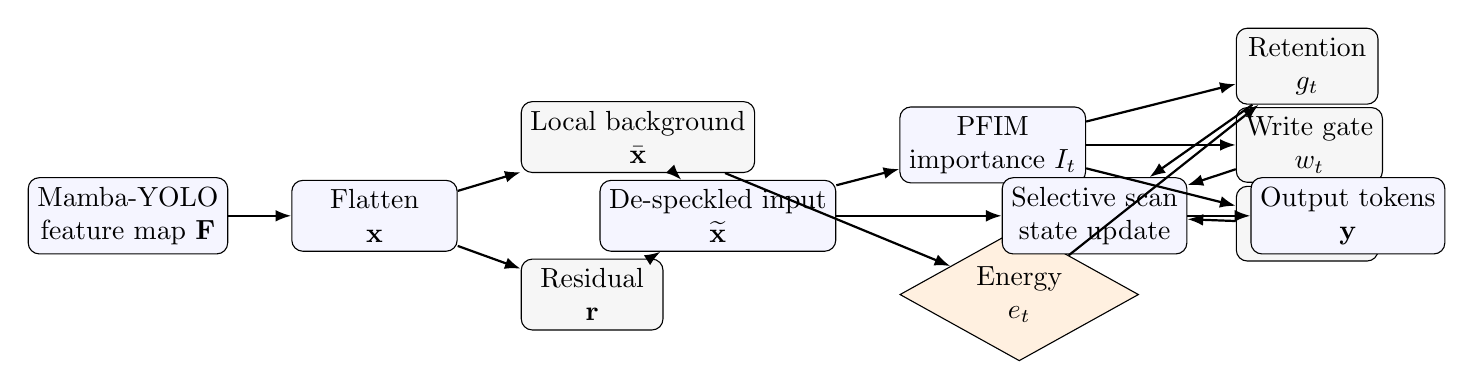
\begin{tikzpicture}[
  node distance=7mm and 8mm,
  block/.style={draw, rounded corners, align=center, minimum height=8mm, minimum width=21mm, fill=blue!4},
  small/.style={draw, rounded corners, align=center, minimum height=7mm, minimum width=18mm, fill=gray!7},
  gate/.style={draw, diamond, aspect=1.8, align=center, minimum height=8mm, fill=orange!12},
  arrow/.style={-{Latex[length=2mm]}, thick}
]
\node[block] (feat) {Mamba-YOLO\\feature map $\mathbf{F}$};
\node[block, right=of feat] (flat) {Flatten\\$\mathbf{x}$};
\node[small, right=of flat, yshift=10mm] (bg) {Local background\\$\bar{\mathbf{x}}$};
\node[small, right=of flat, yshift=-10mm] (res) {Residual\\$\mathbf{r}$};
\node[block, right=18mm of flat] (xt) {De-speckled input\\$\widetilde{\mathbf{x}}$};
\node[block, right=of xt, yshift=9mm] (pfim) {PFIM\\importance $I_t$};
\node[gate, right=of xt, yshift=-10mm] (energy) {Energy\\$e_t$};
\node[small, right=19mm of pfim, yshift=10mm] (gamma) {Retention\\$g_t$};
\node[small, right=19mm of pfim] (write) {Write gate\\$w_t$};
\node[small, right=19mm of pfim, yshift=-10mm] (delta) {Step\\$\Delta_t$};
\node[block, right=21mm of xt] (scan) {Selective scan\\state update};
\node[block, right=of scan] (out) {Output tokens\\$\mathbf{y}$};

\draw[arrow] (feat) -- (flat);
\draw[arrow] (flat) -- (bg);
\draw[arrow] (flat) -- (res);
\draw[arrow] (bg) -- (xt);
\draw[arrow] (res) -- (xt);
\draw[arrow] (xt) -- (pfim);
\draw[arrow] (bg) -- (energy);
\draw[arrow] (pfim) -- (gamma);
\draw[arrow] (pfim) -- (write);
\draw[arrow] (pfim) -- (delta);
\draw[arrow] (energy) -- (gamma);
\draw[arrow] (xt) -- (scan);
\draw[arrow] (gamma) -- (scan);
\draw[arrow] (write) -- (scan);
\draw[arrow] (delta) -- (scan);
\draw[arrow] (scan) -- (out);
\end{tikzpicture}}
\caption{Overall flow of IG-DS-SSM. The module constructs de-speckled inputs and uses PFIM importance to modulate memory retention, state writing, and dynamic transition steps in the selective state-space update.}
\label{fig:ig-ds-ssm-flow}
\end{figure}

\subsection{De-Speckled Input Modeling}

SAR speckle appears as local fluctuations that may be confused with weak ship structures. We estimate a local background representation $\bar{\mathbf{x}}$ using a depth-wise local operator:
\begin{equation}
  \bar{\mathbf{x}} = \mathrm{DWConv}(\mathbf{x}; H,W),
\end{equation}
where the operator is applied on the two-dimensional feature layout. The local residual is
\begin{equation}
  \mathbf{r} = \mathbf{x}-\bar{\mathbf{x}}.
\end{equation}
We then construct a de-speckled input
\begin{equation}
  \widetilde{\mathbf{x}} = \mathbf{x} - \lambda_s \mathbf{r},
  \label{eq:debiased}
\end{equation}
where $\lambda_s$ controls the strength of residual suppression. This operation does not attempt to remove all high-frequency information. Instead, it produces a state-space input whose local disturbance component is attenuated before recurrent propagation.

\subsection{Energy-Aware State Damping}

The local background energy provides a coarse reliability cue. For token $t$, we compute
\begin{equation}
  e_t = \frac{\|\bar{\mathbf{x}}_t\|_2}{\sqrt{C}}.
\end{equation}
The energy term is converted into a soft retention gate
\begin{equation}
  g^{E}_t = g_{\min} + (1-g_{\min})\sigma(-\alpha e_t),
\end{equation}
where $g_{\min}$ prevents complete state erasure and $\alpha$ controls damping strength. High-energy unstable background regions receive stronger damping, reducing the chance that clutter-dominated historical states persist across the scan.

\subsection{Perceptual Feature Importance Module}

Energy alone is insufficient because ship targets may also produce high responses. PFIM estimates a token-level importance score to distinguish target-likely regions from noise-likely regions. Given the de-speckled input, local background, and local statistics, PFIM outputs
\begin{equation}
  I_t = \mathrm{PFIM}(\widetilde{\mathbf{x}}_t,\bar{\mathbf{x}}_t,\mathrm{Std}_{local}(\mathbf{x})_t),
\end{equation}
where $I_t\in[0,1]$. In practice, PFIM is a lightweight branch using local two-dimensional statistics and point-wise transformations, followed by a sigmoid activation. The centered importance is denoted as
\begin{equation}
  \hat{I}_t = I_t - 0.5.
\end{equation}

\subsection{Importance-Guided State Update}

The selective state-space branch generates the input-dependent transition and projection terms from $\widetilde{\mathbf{x}}$. We use PFIM to modulate three update paths.

\paragraph{Memory retention.}
The importance-aware retention gate is
\begin{equation}
  g_t = g_{\min} + (1-g_{\min})\sigma(-\alpha e_t + \beta \hat{I}_t).
  \label{eq:gamma}
\end{equation}
This gate retains more state information around target-likely tokens and suppresses noise-likely propagation.

\paragraph{State writing.}
The write gate controls how strongly the current input enters the state:
\begin{equation}
  w_t = 1 + \rho \tanh(\hat{I}_t),
\end{equation}
\begin{equation}
  \mathbf{u}^{write}_t = w_t \odot \mathbf{u}_t.
\end{equation}

\paragraph{Dynamic transition step.}
PFIM also modulates the transition step:
\begin{equation}
  \Delta_t = \mathrm{softplus}(\Delta^{0}_t + \eta I_t),
\end{equation}
where $\Delta^{0}_t$ is the original transition logit. This allows the model to adjust state evolution speed according to target importance.

The resulting recurrent update can be written conceptually as
\begin{equation}
  \mathbf{h}_t =
  g_t \odot \bar{\mathbf{A}}_t\mathbf{h}_{t-1}
  + \bar{\mathbf{B}}_t\mathbf{u}^{write}_t,
\end{equation}
\begin{equation}
  \mathbf{y}_t = \mathbf{C}_t\mathbf{h}_t + \mathbf{D}\widetilde{\mathbf{x}}_t.
\end{equation}
The residual $\mathbf{D}\widetilde{\mathbf{x}}_t$ preserves current de-speckled evidence outside the recurrent state.

\begin{algorithm}[t]
\caption{IG-DS-SSM Forward Pass}
\begin{algorithmic}[1]
\REQUIRE Tokens $\mathbf{x}\in\mathbb{R}^{N\times C}$ and spatial size $(H,W)$
\STATE Estimate local background $\bar{\mathbf{x}}=\mathrm{DWConv}(\mathbf{x};H,W)$
\STATE Compute residual $\mathbf{r}=\mathbf{x}-\bar{\mathbf{x}}$
\STATE Build de-speckled input $\widetilde{\mathbf{x}}=\mathbf{x}-\lambda_s\mathbf{r}$
\STATE Estimate importance $\mathbf{I}=\mathrm{PFIM}(\widetilde{\mathbf{x}},\bar{\mathbf{x}},\mathrm{Std}_{local})$
\STATE Compute retention gate $g_t$, write gate $w_t$, and transition step $\Delta_t$
\STATE Run selective scan using gated state retention and gated input writing
\STATE Return output tokens $\mathbf{y}$
\end{algorithmic}
\end{algorithm}

\subsection{Decoupled-Gated Extension}

We further study DG-DS-SSM as an extension that explicitly separates erase, write, and transition controls. Its retain/erase branch is
\begin{equation}
  r_t = r_{\min} + (1-r_{\min})\sigma(-\alpha e_t+\beta_e\hat{I}_t),
\end{equation}
the write branch is
\begin{equation}
  q_t = 1+s_w\tanh(\rho_w\hat{I}_t),
\end{equation}
and the delta branch modulates $\Delta_t$ independently. DG-DS-SSM is useful for analysis because it clarifies whether old-state suppression, current-input writing, or transition adaptation contributes most to SAR detection. In our current results, it is competitive but does not surpass the full PFIM-enhanced DS-SSM line; therefore, we treat it as an interpretable extension rather than the main model.

\subsection{Summary of Design Roles}

\begin{table}[h]
\centering
\small
\begin{tabular}{lll}
\toprule
Component & Role & State update effect \\
\midrule
De-speckled input $\widetilde{\mathbf{x}}$ & Suppress local residual disturbance & Cleaner scan input \\
Energy $e_t$ & Estimate unreliable background strength & Damps noisy state retention \\
PFIM importance $I_t$ & Estimate target-likely tokens & Protects useful target response \\
Retention gate $g_t$ & Modulate historical memory & Controls state carry-over \\
Write gate $w_t$ & Modulate current input writing & Controls state injection \\
Step $\Delta_t$ & Modulate transition sensitivity & Controls state evolution speed \\
\bottomrule
\end{tabular}
\caption{Functional roles of the IG-DS-SSM components.}
\label{tab:roles}
\end{table}

\end{document}
